\subsection{Solve Rates Stagnate as Cost Grows}
\label{sec:overall-results}

\begin{table}[t]
\centering
\caption{Per-model performance on \scb{}. For each model we report its best just-solve run, ranked by isolated solve rate with core, strict, and \$/checkpoint as tiebreakers. Solve rates use a fixed 196-checkpoint denominator; missing checkpoints count as unsolved. Other metrics are only for ran checkpoints. \textbf{Bold} marks the best value per column. See \autoref{tab:performance-appendix} for the full set of runs.}
\label{tab:performance-overview}
\small
\setlength{\tabcolsep}{4pt}
\resizebox{\textwidth}{!}{%
\begin{tabular}{l | rrrr | rrr | rr}
\toprule
 & \multicolumn{4}{c|}{Solve Rate (\%)}
 & \multicolumn{3}{c|}{Cost \& Time}
 & \multicolumn{2}{c}{Quality} \\
\cmidrule(lr){2-5} \cmidrule(lr){6-8} \cmidrule(l){9-10}
Model & Strict & Iso. & Core & Partial & \$/CKPT & Net \$ & Min/CKPT & Erosion & Verbosity \\
\midrule
Opus 4.5 & 9.2 & 17.3 & 57.7 & 25.0 & 2.53{\scriptsize$\pm$1.57} & 492.40 & 7.2{\scriptsize$\pm$3.7} & 0.70{\scriptsize$\pm$0.20} & 0.43{\scriptsize$\pm$0.18} \\
Opus 4.6 & 9.7 & 20.9 & \textbf{67.3} & 27.8 & 3.17{\scriptsize$\pm$2.82} & 620.80 & 13.1{\scriptsize$\pm$12.9} & 0.75{\scriptsize$\pm$0.15} & 0.44{\scriptsize$\pm$0.19} \\
Opus 4.7 & 8.2 & 20.9 & 65.8 & 36.1 & 2.17{\scriptsize$\pm$1.83} & 425.34 & 6.8{\scriptsize$\pm$5.0} & 0.76{\scriptsize$\pm$0.17} & 0.48{\scriptsize$\pm$0.21} \\
Sonnet 4.6 & 7.1 & 16.8 & 57.7 & 27.8 & 1.96{\scriptsize$\pm$1.97} & 383.83 & 14.2{\scriptsize$\pm$14.2} & 0.75{\scriptsize$\pm$0.20} & 0.44{\scriptsize$\pm$0.19} \\
\midrule
GPT~5.2 Codex & 9.7 & 21.9 & 56.1 & 36.1 & 0.85{\scriptsize$\pm$0.80} & 167.29 & 12.3{\scriptsize$\pm$9.7} & 0.73{\scriptsize$\pm$0.18} & 0.50{\scriptsize$\pm$0.16} \\
GPT~5.3 Codex & 11.2 & 26.0 & 60.7 & 41.7 & 0.66{\scriptsize$\pm$0.49} & 129.65 & 7.7{\scriptsize$\pm$4.6} & 0.64{\scriptsize$\pm$0.19} & 0.46{\scriptsize$\pm$0.18} \\
GPT~5.3 Spark & 3.1 & 8.2 & 29.1 & 11.1 & \textbf{0.20{\scriptsize$\pm$0.41}} & \textbf{37.17} & \textbf{2.4{\scriptsize$\pm$4.6}} & 0.68{\scriptsize$\pm$0.19} & 0.48{\scriptsize$\pm$0.16} \\
GPT~5.4 & 10.7 & 23.5 & 62.8 & 36.1 & 0.72{\scriptsize$\pm$0.51} & 141.32 & 8.0{\scriptsize$\pm$4.7} & 0.51{\scriptsize$\pm$0.19} & 0.33{\scriptsize$\pm$0.13} \\
GPT~5.4 Mini & 5.1 & 13.8 & 53.1 & 22.2 & 0.45{\scriptsize$\pm$0.35} & 89.03 & 6.2{\scriptsize$\pm$3.8} & 0.66{\scriptsize$\pm$0.17} & 0.42{\scriptsize$\pm$0.12} \\
GPT~5.5 & \textbf{14.8} & \textbf{28.1} & 66.8 & \textbf{50.0} & 1.51{\scriptsize$\pm$0.81} & 295.59 & 6.0{\scriptsize$\pm$2.4} & \textbf{0.49{\scriptsize$\pm$0.20}} & \textbf{0.32{\scriptsize$\pm$0.12}} \\
\midrule
Composer~2 & 6.1 & 16.3 & 52.6 & 13.9 & 0.44{\scriptsize$\pm$0.44} & 86.31 & 8.8{\scriptsize$\pm$8.3} & 0.72{\scriptsize$\pm$0.15} & 0.45{\scriptsize$\pm$0.17} \\
GLM~5.1 & 9.7 & 13.8 & 40.3 & 30.6 & 1.47{\scriptsize$\pm$1.45} & 288.85 & 31.4{\scriptsize$\pm$20.0} & 0.71{\scriptsize$\pm$0.17} & 0.41{\scriptsize$\pm$0.18} \\
Kimi~K2.5 & 4.6 & 9.7 & 39.8 & 19.4 & 0.33{\scriptsize$\pm$0.25} & 63.21 & 14.5{\scriptsize$\pm$10.0} & 0.72{\scriptsize$\pm$0.20} & 0.44{\scriptsize$\pm$0.20} \\
Kimi~K2.6 & 10.7 & 18.9 & 51.0 & 33.3 & 0.74{\scriptsize$\pm$0.64} & 133.18 & 26.9{\scriptsize$\pm$20.7} & 0.76{\scriptsize$\pm$0.20} & 0.51{\scriptsize$\pm$0.22} \\
MiniMax~M2.7 & 2.0 & 4.1 & 28.1 & 8.3 & 0.34{\scriptsize$\pm$0.23} & 65.79 & 11.9{\scriptsize$\pm$6.8} & 0.73{\scriptsize$\pm$0.16} & 0.47{\scriptsize$\pm$0.17} \\
\bottomrule
\end{tabular}%
}
\end{table}

\autoref{tab:performance-overview} summarizes solve rates across \overallNumModels{} models on \scb. No agent \emph{fully} solves any of the \transProblems{} problems. No run passes every test at every checkpoint end-to-end. \textbf{\overallBestModel{}} achieves the highest strict solve rate at \overallBestStrictSolveRate{}\% and isolated solve rate peaks at \overallIsoSolveMax{}\%. Opus 4.5 achieves the highest core solve rate at \overallCoreSolveMax{}\%.
\begin{figure}[t]
    \centering
    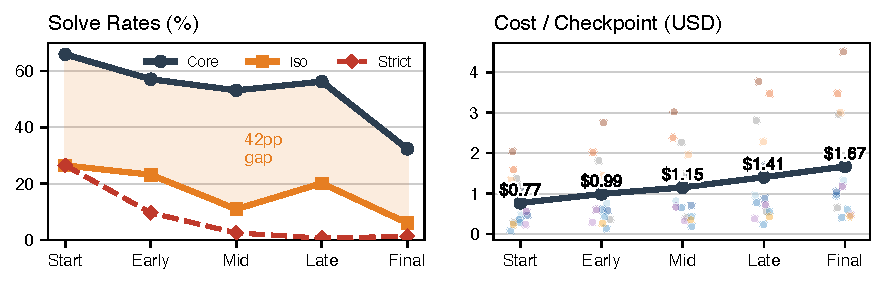
\includegraphics[width=\textwidth]{figures/overview_solve_cost.pdf}
    \caption{\textbf{Performance degrades as problems progress and cost per checkpoint steadily rise.} \emph{Left:} Checkpoint solve rate by type. \emph{Right:} Mean cost per checkpoint as problems progress.}
    \label{fig:solve-cost}
\end{figure}

\autoref{fig:solve-cost} shows the gap between core and isolated pass rates widens from \abFigCoreIsoRatioMin{}$\times$ to \abFigCoreIsoRatioMax{}$\times$. Core pass rate falls from \overallTestCorePassEarlyPct{}\% to \overallTestCorePassLatePct{}\%. Functionality pass rate changes by less than six points, from \overallTestFuncPassEarlyPct{}\% to \overallTestFuncPassLatePct{}\%, while error pass rate drops from \overallTestErrorPassEarlyPct{}\% to \overallTestErrorPassLatePct{}\%.

Cost and context grow while code movement declines. Mean cost per checkpoint grows \abFigCostGrowth{}$\times$ from the start to end, while mean relative lines changed fall from \overallChurnMeanEarlyPct{}\% early to \overallChurnMeanLatePct{}\% late. Total recorded token accounting is \overallTokensTotalB{}B tokens. Normalized to 196 checkpoints, \overallTokenLowestModel{} has the lowest token spend at \overallTokenLowestNormB{}B tokens, while \overallTokenHighestModel{} has the highest at \overallTokenHighestNormB{}B tokens. 